\documentclass[a4paper,11pt]{article}

\usepackage[left=2cm, top=3cm, text={17cm, 24cm}]{geometry}
\usepackage[czech]{babel}
\usepackage[utf8]{inputenc}
\usepackage{times}
\usepackage[unicode]{hyperref}
\hypersetup{colorlinks = true, hypertexnames = false}

\usepackage{graphicx}
\graphicspath{ {./img/} }

\begin{document}
	\begin{titlepage}
		\begin{center}
			\textsc{\Huge Vysoké učení technické v~Brně\\
				\vspace{0.4em}\huge Fakulta informačních technologií}
			
			\vspace{\stretch{0.382}}
			
			{\LARGE Umělá inteligence a strojové učení\\
				\Huge Umělá inteligence pro hru Dicewars\\ \vspace{0.3em}}
			
			\vspace{\stretch{0.618}}
			
			{\Large \hfill Martin Kostelník (xkoste12)\\ \hfill Ivo Meixner (xmeixn00)\\ \today \hfill Michal Dostál (xdosta51)}
		\end{center}
	\end{titlepage}

	\section{Úvod}
		Cílem tohoto projektu je vytvořit umělou inteligenci pro hru Dicewars\footnote{\url{https://github.com/ibenes/dicewars}}. Dicewars je tahová hra pro dva a více hráčů s úplnou informací o prostředí (nebereme-li v potaz rezervy) a s nedeterministickým výsledkem útoků. V rámci projektu uvažujeme pouze hry čtyř hráčů. Dokumentace je rozdělena do dvou hlavních částí. První, kapitola \ref{section:search}, pojednává o prohledávání stavového prostoru. Kapitola \ref{section:nn} popisuje heuristickou funkci využitou k ohodnocování stavů hry.
		
	\section{Prohledávání stavového prostoru}
	\label{section:search}
		Jedním z velice známých algoritmů pro prohledávání stavových prostorů ve hrách je \texttt{MiniMax}. Ten ale předpokládá deterministické akce, což zde nemáme. Rozšířením pro nedeterminismus je algoritmus\\\texttt{ExpectiMiniMax}. Oba algoritmy jsou pouze pro hry dvou hráčů. Naše řešení vždy očekává hru, ve které budou hráči čtyři. K prohledávání stavového prostoru her ve hrách více hráčů se dá využít algoritmus \texttt{$Max^n$}. Algoritmus \texttt{$Max^n$} je tedy zobecněním algoritmu \texttt{MiniMax} pro více než dva hráče. V této kapitole se podíváme, jak funguje a jak byl v projektu implementován.
		
	\subsection{Algoritmus \texttt{$Max^n$}}
		V \texttt{MiniMax} je ohodnocením stavů jedno číslo. Jeden hráč se snaží číslo maximalizovat, druhý naopak minimalizovat. Pokud přidáme hráčů více, jedno číslo pro ohodnocení stavů nám už nestačí. Použije se proto $n$-tice, kde $n$ značí počet hráčů. Každý hráč se poté snaží maximalizovat své vlastní číslo. To je ilustrováno na obrázku \ref{fig:maxn}. V praxi to funguje tak, že prohledáváme pouze do omezené hloubky. Všechny stavy v maximální hloubce ohodnotíme heuristickou funkcí a následně je každému rodičovskému stavu přiřazeno odpovídající ohodnocení vzhledem k tomu, který hráč je na řadě.
		
		\begin{figure}[h]
			\centering
			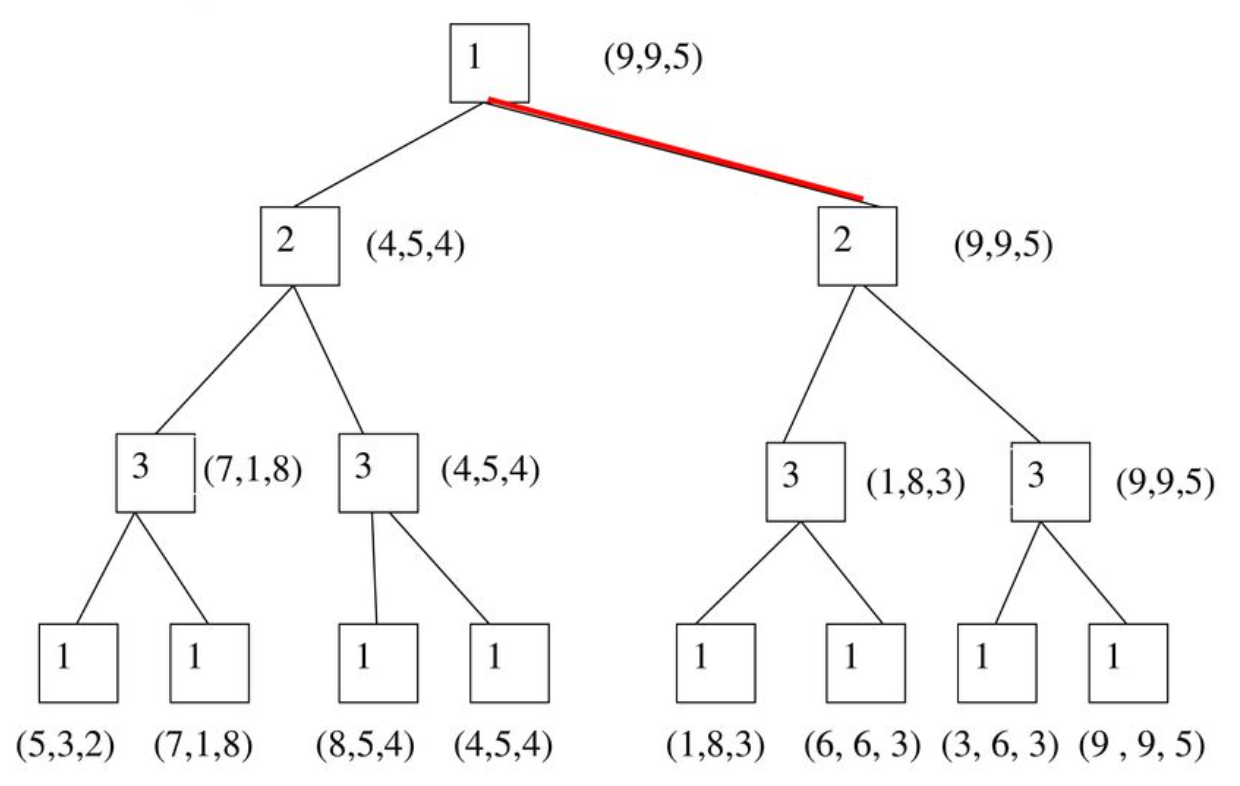
\includegraphics[scale=0.5]{maxn.png}
			\caption{Ukázka algoritmu \texttt{$Max^n$} pro tři hráče. Převzato z \url{https://slideplayer.com/slide/15266490/}}
			\label{fig:maxn}
		\end{figure}
		
	\subsection{Implementace}
		Algoritmus je implementován jako rekurzivní funkce \texttt{maxn()}, která má na vstupu aktuální stav herní plochy, počet již provedených přesunů a aktuální hloubku. Funkce vrací dvojici, kde první prvek je ohodnocení aktuálního stavu a druhý prvek nejlepší nalezený tah. Funkce nejprve nalezne všechny možné tahy (útoky i přesuny, pokud přesunů nebylo provedeno maximální množství). Funkce následně prochází všechny možné tahy na aktuální úrovni kromě útoků s pravděpodobností úspěchu menší než 50 \%. Tyto tahy jsou simulovány na kopii herní plochy, nad kterou je následně rekurzivně volána funkce \texttt{maxn()}. Útoky se vždy simulují jako úspěšné.
		Pokud je ohodnocení stavu po provedení simulace příznivější než aktuální, tah si zapamatujeme.
		
		Stavový prostor je velice rozsáhlý, zejména pokud bereme v potaz i přesuny. Maximální hloubku prohledávání jsme omezili následovně:
		\begin{itemize}
			\item 3 -- pokud zbývá více než 10 sekund
			\item 2 -- pokud zbývá více než 2 sekundy
			\item 1 -- jinak
		\end{itemize}
	
		Nechtěli jsme přidávat přílišnou logiku pro filtrování lidsky nepříliš logicky vypadajících tahů, abychom neomezovali model strojového učení.
		
		Před vytvořením modelu jsme pro ohodnocení stavu využili naivní funkci, která spočítá pravděpodobnost výhry každého hráče podle podílu jeho kostek vůči celkovému počtu kostek na herní ploše. Ta je implementována jako \texttt{evaluate\_state()}. Ve finálním řešení není vůbec použita.
	
	\section{Neuronová síť pro aproximaci heuristické funkce}
	\label{section:nn}
		Pro prohledávání stavů pomocí \texttt{$Max^n$} algoritmu je nutné vytvořit heuristickou funkci pro ohodnocení jednotlivých stavů. Tuto funkci jsme se rozhodli aproximovat s využitím neuronové sítě. K dosažení tohoto cíle jsou zapotřebí několik kroků, které jsou dále popsány v této sekci.
		
		Vytvořená neuronová síť se skládá celkem z tří lineární vrstev a dvou \texttt{dropout} vrstev. První dvě lineární vrstvy používají aktivační funkci \texttt{ReLU}. Pravděpodobnost v \texttt{dropout} vrstvách byla nastavena na hodnotu $0.5$. Popis architektury získaný pomocí pomocné funkce knihovny \texttt{PyTorch} je ilustrován na \ref{fig:model}.
		
		Při implementaci a experimentaci s modelem jsme narazili na problém ohledně aktivační funkce poslední lineární vrstvy. Nejprve jsme zvolili aktivační funkci \texttt{softmax}, aby výsledná $n$-tice reprezentovala\\pravděpodobnost výhry každého hráče. Stávalo se ale, že funkce velice často začala vracet $n$-tice s jedním elementem s hodnotou $1$ a ostatní v nule. Pokud toto nastalo, nebyli jsme schopni vybrat lepší tah. Stejný problém nastal u aktivační funkce \texttt{log\_softmax}. Nakonec jsme se rozhodli nechat poslední vrstvu čistě lineární, bez jakékoliv aktivační funkce. Výstupem je tak $n$-tice, kde každý prvek představuje skóre každého hráče. Tato hodnota není nijak omezena shora ani zdola a nikdy se tak nestane, že bychom nebyli schopni najít lepší tah.
		
		\begin{figure}[h]
			\centering
			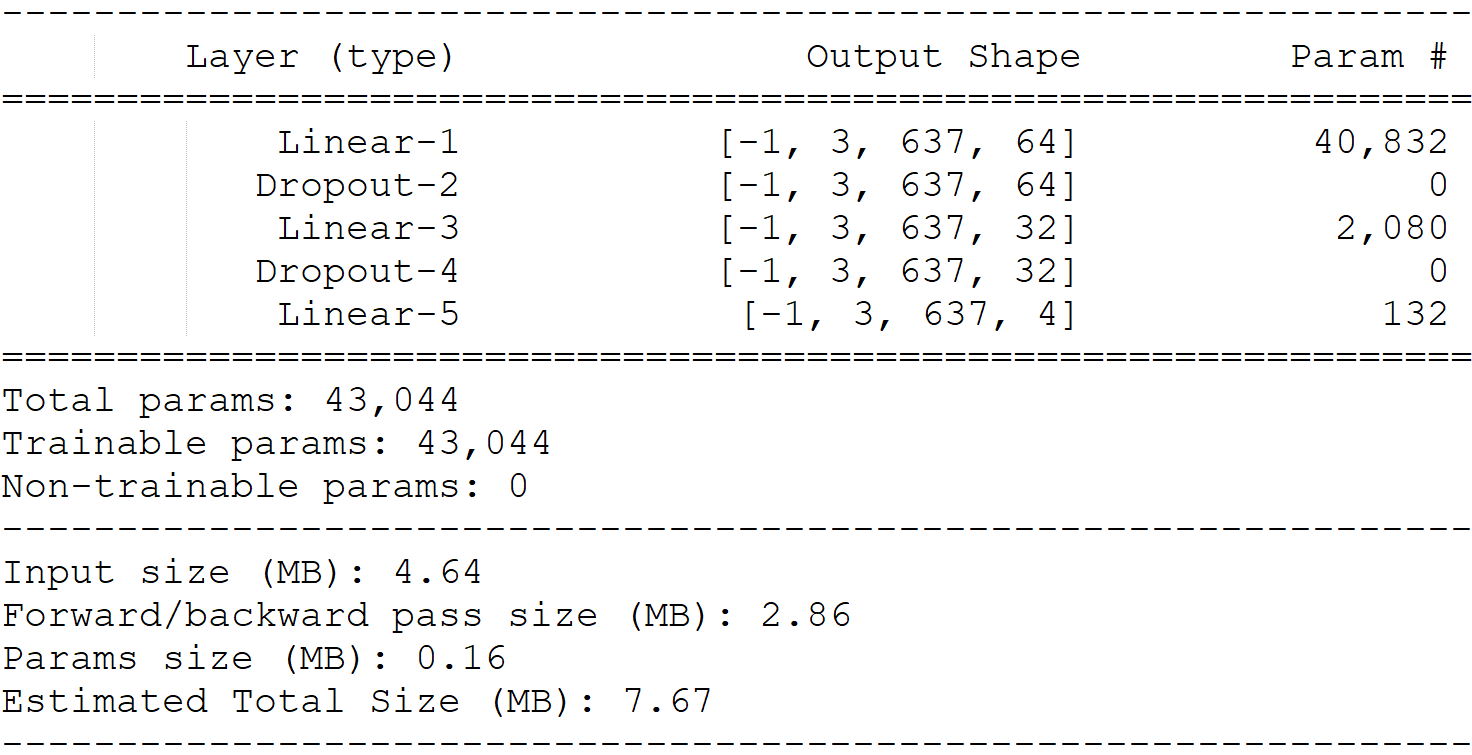
\includegraphics[scale=0.5]{model.png}
			\caption{Architektura modelu neuronové sítě.}
			\label{fig:model}
		\end{figure}
	
	\subsection{Serializace stavu hry}
	\label{serialization}
		Pro optimalizaci velikosti souborů reprezentujících průběh hry je informace o jejím vítězi a sousednosti herních políček uložena na disku pouze jednou, společně pro všechny stavy herního pole, které během hry nastaly. Serializace do tohoto formátu se provádí při generování trénovacích dat.
		
		Na disku je každá hra reprezentována objektem typu \texttt{tuple} složeným ze tří hodnot:
	
		\begin{itemize}
			\item Vítěz hry zakódovaný v one-hot formátu jako pole čtyř hodnot typu \texttt{int},
			\item Jednorozměrné pole popisující sousednost herních políček typu \texttt{list} s prvky typu \texttt{int}, kde 0 označuje dvojici políček, které spolu nesousedí, a 1 značí dvě sousední políčka.
			\item Pole typu \texttt{list} obsahující jednotlivé stavy hry v pořadí, ve kterém nastaly, přičemž jednotlivé prvky tohoto pole mají následující formát:
			\begin{itemize}
				\item One-hot zakódovaná informace o hráči, který je aktuálně na tahu,
				\item Jednorozměrné pole popisující vlastníky jednotlivých herních políček, kde je pro každé políčko jedna hodnota typu \texttt{int} obsahující index hráče od 1 do 4,
				\item Jednorozměrné pole obsahující počet kostek na jednotlivých herních políčcích uložených v typu \texttt{int} od 1 do 8,
				\item Jednorozměrné pole s velikostmi největších oblastí jednotlivých hráčů v typu \texttt{int} od 0 do 34.
			\end{itemize}
		\end{itemize}
	
		Jako vstup neuronové sítě se používá jednorozměrné pole složené z hodnot popisující stav herní plochy rozšířené o pole popisující sousednost herních políček. Vstupní pole má tedy celkem 637 prvků, čímž je kompletně popsán aktuální stav hry. Vítěz je v one-hot kódování použit jako výstup neuronové sítě při trénování. Funkce pro serializaci při běhu hry jsou uloženy v souboru \texttt{utils.py}.
	
		\subsection{Generování trénovacích dat}
		Data pro trénování byla vygenerována pomocí upravené verze hry DiceWars, která se nachází v adresáři \texttt{dicewars/supp\_xkoste12/generator/}. Většina důležitých změn byla provedena v souboru\\\texttt{dicewars/server/game.py}, kde bylo přidáno zaznamenávání stavů hry na začáku hry a následně po každém tahu každého hráče. Tyto stavy jsou na konci hry doplněny o pole popisující sousednost herních políček a informaci o výherci dané hry zakódované v one-hot formátu. Výsledná data jsou uložena na disk do adresáře \texttt{dicewars/supp\_xkoste12/data/} v populárním Pythonovém serializačním formátu \emph{pickle}. Přesnější popis formátu serializovaných dat se nachází v sekci \ref{serialization}. Histogram délky vygenerovaných her použitých při trénování lze vidět na obrázku \ref{fig:gamelen}.
		
		Pro spuštění generátoru je nutné být v jeho kořenovém adresáři\\(\texttt{dicewars/supp\_xkoste12/generator/}), spustit skript \texttt{install.sh} a aktivovat virtuální prostředí příkazem \texttt{source path.sh}. Samotný generátor se spouští v podobě skriptu \texttt{gen.sh}. Pro zastavení tohoto skriptu stačí vytvořit v kořenovém adresáři generátoru soubor s názvem \texttt{stop}, například příkazem \texttt{touch stop}.
		
		\begin{figure}[h]
			\centering
			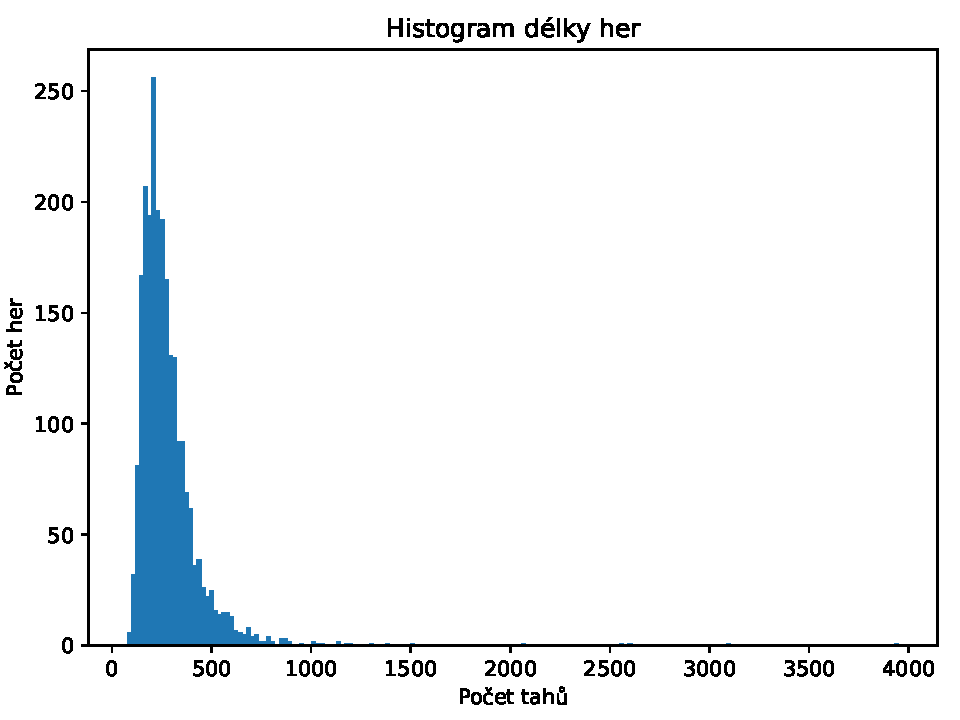
\includegraphics[scale=0.7]{game_len_hist.pdf}
			\caption{Histogram délky her.}
			\label{fig:gamelen}
		\end{figure}
	
	\subsection{Trénování modelu}
		Pro natrénování modelu bylo vygenerováno celkem $2250$ her, ze kterých jsme získali $638 255$ různých stavů herní plochy. Tato data byla následně rozdělena na trénovací a validační datovou sadu. Trénovací sada obsahuje 80 \% z původních dat. Validační sata zbylých 20 \%. Bylo nutné vytvořit třídu \texttt{GameDataSet}, která implementuje funkce \texttt{\_\_len\_\_()} a \texttt{\_\_getitem\_\_()}. Tyto funkce poté používá třída \texttt{torch.DataLoader}, která data zamíchá a rozdělí do skupin o velikosti $256$.
		
		Jako optimalizační algoritmus jsme zvolili algoritmus \texttt{Adam} s \texttt{learning rate} s hodnotou $0.01$. Pro \texttt{loss} funkci jsme zvolili \texttt{CrossEntropy}. Počet epoch trénování jsme nastavili na $1000$ s tím, že nový model se uloží pouze tehdy, pokud validační loss dosáhne nového minima. Nejlepší model jsme získali v epoše číslo $330$. Průběh loss funkce pro trénovací i validační data lze vidět na obrázku \ref{fig:loss}. Veškeré trénování probíhalo na stolním počítači s grafickou kartou nVidia RTX 3070.
		
		\begin{figure}[h]
			\centering
			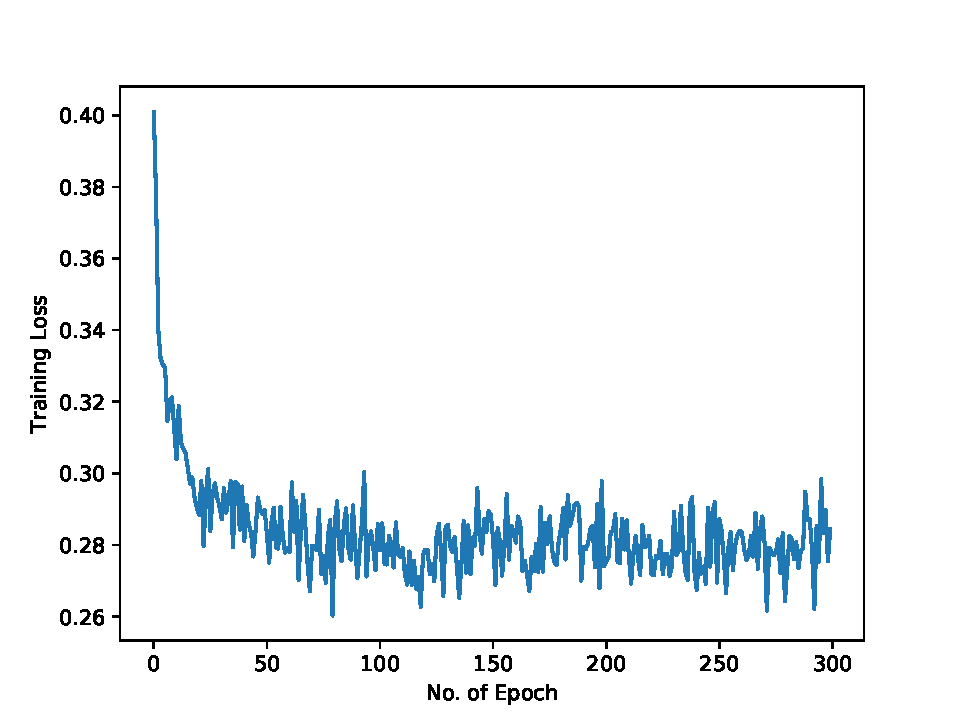
\includegraphics[scale=0.5]{training_loss.pdf}
			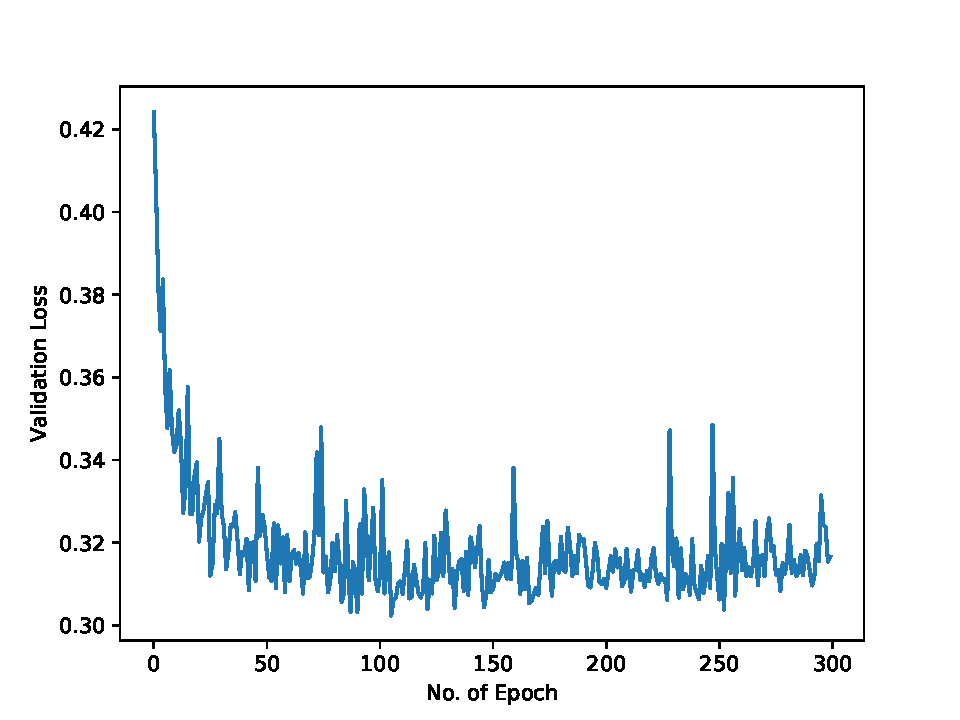
\includegraphics[scale=0.5]{valid_loss.pdf}
			\caption{Průběh trénovací a validační loss funkce během trénování.}
			\label{fig:loss}
		\end{figure}
	
	\subsection{Použití modelu}
		V hlavním souboru s implementací umělé inteligence je vytvořena nová heuristická funkce\\\texttt{evaluate\_state\_nn()}, která dostane aktuální stav herní plochy serializuje jej jak je popsáno v \ref{serialization} a vrátí její ohodnocení. V inicializační funkci třídy je třeba model nejprve načíst a vyhodnotit. Načtení vyžaduje přístup k třídě popisující neuronovou síť. Zkopírovali jsme potřebný kód do souboru \texttt{utils.py} abychom předešli problémům s importem ze složky \texttt{supp-xkoste12}. Další problémy se projevili, když jsme se snažili model spouštět na grafické kartě. Nejjednodušším způsobem bylo toto zakázat a používat pouze procesor.
	
	\section{Obsah archivu}
		Odevzdaný archiv obsahuje následující:
		
		\begin{itemize}
			\item \texttt{xkoste12.pdf} - Dokumentace projektu.
			\item \texttt{supp-xkoste12/data} -- Adresář obsahující vzorek dat použitých ke trénování.
			\item \texttt{supp-xkoste12/generator} -- Adresář obsahující změněný kód použitý při generování trénovacích dat.
			\item \texttt{supp-xkoste12/model.py} -- Skript použitý pro natrénování modelu neuronové sítě.
			\item \texttt{xkoste12/model.pth} -- Natrénovaný model neuronové sítě pro aproximaci heuristické funkce.
			\item \texttt{xkoste12/xkoste12.py} -- Skript obsahující definici třídy \texttt{AI}.
			\item \texttt{xkoste12/utils.py} -- Skript obsahující architekturu neuronové sítě a funkce pro serializaci stavu hry.
		\end{itemize}
		
	\section{Závěr}
	V projektu byla implementována umělá inteligence pro hru Dicewars využívající algoritmus \texttt{$Max^n$} s měnící se maximální hloubkou dle zbývajícího času. Dále byla vytvořena a natrénována neuronová síť pro ohodnocení jednotlivých stavů. Vytvoření modelu zahrnovalo úpravu původní verze hry pro vygenerování trénovacích dat, trénování modelu a jeho integraci do prohledávání stavového prostoru.
	
	Výsledná umělá inteligence dosahuje výsledků podobných jako implementace v modulu \texttt{dt}, avšak na implementace v modulu \texttt{kb} nestačí. Výsledek turnaje o sto hrách lze vidět na obrázku \ref{fig:winrate}.
	
	\begin{figure}[ht]
		\centering
		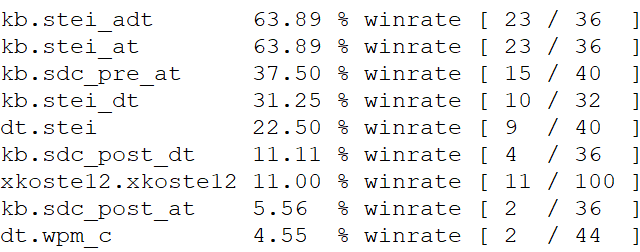
\includegraphics[scale=0.7]{winrate.png}
		\caption{Výsledek turnaje o sto hrách.}
		\label{fig:winrate}
	\end{figure}
	
	Při testování jsme si všimli zajímavé věci. Pořadí hráčů značně ovlivňuje jejich šance na výhru. Hráč, který začíná, je na tom vždy lépe než druhý, ten lépe než třetí a tak dále. To lze vidět na obrázku \ref{fig:order}. Spuštění velkého množství her by mělo tuto skutečnost vyvážit, ale člověk musí být opatrný při spouštění malého množství při testování funkčnosti.
	
	\begin{figure}[ht]
		\centering
		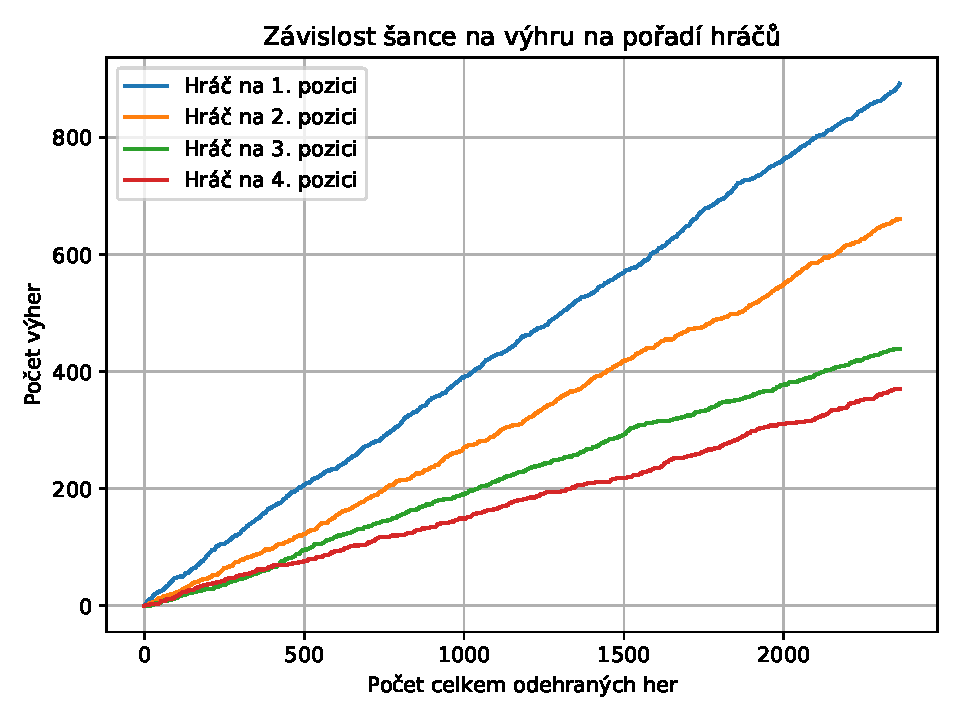
\includegraphics[scale=0.65]{win_prob.pdf}
		\caption{Graf zobrazující závislost šance na výhru na pořadí hráčů.}
		\label{fig:order}
	\end{figure}
	
\end{document}